\section{\texorpdfstring{Popis logické funkce}{Popis logicke funkce}}

% =====================================================================================================================
	\begin{frame}
    \frametitle{Logický obvod - logická funkce}
		
		
		\begin{center}
			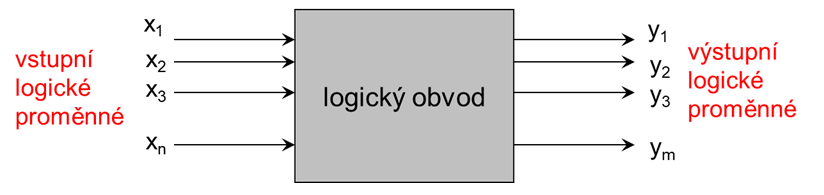
\includegraphics[width=0.7\textwidth]{fig/logicky_obvod.png}
		\end{center}
		
		
		\begin{itemize}
			\item vstupy a výstupy nabývají pouze logických hodnot, tj. 0 a 1
			\item rozlišujeme:
			
			\begin{itemize}
				\item \textbf{kombinační logické obvody}, kde je výstupní hodnota dána výhradně aktuální hodnotou vstupů a
				\item \textbf{sekvenční logické obvody}, kde je výstupní hodnota navíc dána i předchozím stavem vstupů a výstupů (přítomnost paměti, zpětné vazby apod.).
			\end{itemize}
			
		\end{itemize}
		
	\end{frame}
	
% =====================================================================================================================
	\begin{frame}
    \frametitle{Kombinační logika}
		\boldmath
		
		\begin{itemize}
			\item je plně určena funkčním chováním: $y_i = f(x_0, x_1 ..., x_n)$
			\item neobsahuje paměť, tedy \textbf{\textcolor{blue}{nemá možnost}} plnit funkci aplikace, kde je například nutné \textbf{\textcolor{blue}{uložit stav}} systému. \\ \vspace{3pt}
			\textbf{Příklad:} START/ STOP tlačítka v laboratoři uchovávají stav o zapnutí a vypnutí napájení.
			\item skutečný obvod může obsahovat parazitní časové závislosti, nejčastěji je to zpoždění dané:
			
			\begin{itemize}
				\item elektrickou kapacitou součástek,
				\item délkou přívodních vodičů (indukčnost, vlna na vedení),
				\item zatížením výstupu logického prvku apod.
			\end{itemize}
			
			Nejčastějšími důsledky uvedeného jsou pak:
			
			\begin{itemize}
				\item zkreslení hran signálů a
				\item hazardy.
			\end{itemize}
		\end{itemize}
		
	\end{frame}
	
% =====================================================================================================================
	\begin{frame}
    \frametitle{Logická funkce}
		\boldmath
		
		\begin{itemize}
			\item Jde o zobrazení $N$ vstupních prvků nabývajících hodnot 0 nebo 1 na jednu výstupní hodnotu 0 nebo 1.
			
			\begin{itemize}
				\item Celkový počet kombinací vstupních hodnot: $2^N$
				\item Celkový počet různých funkcí: $2^{(2^N)}$
			\end{itemize}
			
			\vspace{5mm}
			\item Zápis logické funkce:
			
			\begin{enumerate}
				\item úplná disjunktivní normální forma (Sum of Products – SOP), což je součet součinnů,
				
				\begin{center}
					$Y = (\bar{A} \cdot \bar{B}) + (B\cdot C) + (A\cdot B)$
				\end{center}
				
				\item úplná konjunktivní normální forma (Product of Sums - POS), což je součin součtů.
				
				\begin{center}
					$Y = (\bar{A} + B) \cdot (A + \bar{B} + C)$
				\end{center}
				
			\end{enumerate}
		\end{itemize}
		
	\end{frame}
	
% =====================================================================================================================
	\begin{frame}
    \frametitle{Booleova algebra}
		\boldmath
		
		
		\begin{itemize}
			\item Pracuje s dvouhodnotovou logikou,
			\item Využívá tři základní operace:
			
			\begin{enumerate}
				\item logický součin - AND, značíme symbolem součinu,
				\item logický součet - OR, značíme symbolem součtu,
				\item logickou negaci - NOT, značíme čárkou nad proměnnou.
			\end{enumerate}
			
		\end{itemize}
		\vspace{5mm}
		
		\begin{minipage}[t][0.4\textheight][t]{0.32\textwidth}
      \textbf{AND}
			
			\begin{itemize}
				\item minterm
				\item musí plati oba
			
      
				\begin{tabular}{ c c | c}
					A & B & Y \\
					\hline
					0 & 0 & 0 \\
					0 & 1 & 0 \\
					1 & 0 & 0 \\
					1 & 1 & 1 \\
				\end{tabular}
			\end{itemize}
      
		\end{minipage}
		\begin{minipage}[t][0.4\textheight][t]{0.4\textwidth}
      \textbf{OR}
			
			\begin{itemize}
				\item maxterm
				\item platí alespoň jeden
      
				\begin{tabular}{ c c | c}
					A & B & Y \\
					\hline
					0 & 0 & 0 \\
					0 & 1 & 1 \\
					1 & 0 & 1 \\
					1 & 1 & 1 \\
				\end{tabular}
			\end{itemize}
      
		\end{minipage}
		\begin{minipage}[t][0.4\textheight][t]{0.25\textwidth}
      \textbf{NOT}
			
			\begin{itemize}
				\item inverze
				\vspace{5mm}
      
				\begin{tabular}{ c | c}
					A & Y \\
					\hline
					0 & 1 \\
					1 & 0 \\
				\end{tabular}
			\end{itemize}
      
		\end{minipage}
		
	\end{frame}
	
% =====================================================================================================================
	\begin{frame}
    \frametitle{Booleova algebra - zákony}
		\boldmath
		
		\begin{tabular}{ p{5cm} l l}
			\textbf{Identita:} & $A + 0 = A$ & $A\cdot 1 = A$ \\
			\textbf{Agresivita jedničky a nuly:} & $A + 1 = 1$ & $A\cdot 0 = 0$ \\
			\textbf{Vyloučení třetího, inverze:} & $A + \bar{A} = 1$ & $A\cdot \bar{A} = 0$ \\
			\textbf{Dvojitá negace:} & $\bar{\bar{A}} = A$ & \\
			\textbf{Komutativita:} & $A + B = B + A$ & $A\cdot B = B \cdot A$ \\
		\end{tabular}
		
		\vspace{4mm}
		\begin{tabular}{ p{5cm} l}
			\textbf{Asociativita:} & $(A + B) + C= A + (B + C)$  \\
														 & $(A \cdot B) \cdot C= A \cdot (B \cdot C)$  \\
			\textbf{Distributivita:} & $(A + B) \cdot C= (A\cdot C) + (B \cdot C)$  \\
														 & $(A \cdot B) + C= (A+C) \cdot (B + C)$  \\
		\end{tabular}
		
		\vspace{4mm}
		\begin{tabular}{ p{5cm} l}
			\textbf{Absorpce:} & $A \cdot (A + B) = A$  \\
												 & $A + (A \cdot B) = A$  \\
			\textbf{Absorpce negace:} & $A \cdot (\bar{A} + B) = A \cdot B$  \\
												 & $A + (\bar{A} \cdot B) = A + B$  \\
		\end{tabular}

	\end{frame}
	
% =====================================================================================================================
	\begin{frame}
    \frametitle{Booleova algebra - De Morganovy zákony}
		\boldmath
		
		
		\begin{enumerate}
			\item Když není splněna platnost alespoň jednoho, pak neplatí ani jeden
			\begin{center}
				$\overline{A + B} = \bar{A}\cdot \bar{B}$
			\end{center}
			
			
			\item Když není splněna platnost obou současně, pak alespoň jeden z nich neplatí
			\begin{center}
				$\overline{A \cdot B} = \bar{A}+ \bar{B}$
			\end{center}
		\end{enumerate}
		
		\vspace{5mm}
		\begin{minipage}[t][0.4\textheight][t]{0.45\textwidth}
      \textbf{Ad 1}
			
				\begin{tabular}{ c c | c c }
					$A$ & $B$ & $\bar{A} + \bar{B}$ & $A \cdot B$\\
					\hline
					0 & 0 & 1 & 0 \\
					0 & 1 & 1 & 0 \\
					1 & 0 & 1 & 0 \\
					1 & 1 & 0 & 1 \\
				\end{tabular}
      
		\end{minipage}
		\begin{minipage}[t][0.4\textheight][t]{0.45\textwidth}
      \textbf{Ad 2}
			
				\begin{tabular}{ c c | c c }
					$A$ & $B$ & $\bar{A} \cdot \bar{B}$ & $A + B$\\
					\hline
					0 & 0 & 1 & 0 \\
					0 & 1 & 0 & 1 \\
					1 & 0 & 0 & 1 \\
					1 & 1 & 0 & 1 \\
				\end{tabular}
      
		\end{minipage}

	\end{frame}

% =====================================================================================================================
	\begin{frame}
    \frametitle{Popis logické funkce - pravdivostní tabulka}
		\boldmath
		
		\begin{minipage}[t][\textheight][t]{0.45\textwidth}
		\vspace{10mm}
		\begin{center}
			\begin{tabular}{ c c c | c }
				$A$ & $B$ & $C$ & $Y$\\
				\hline
				0 & 0 & 0 & 0 \\
				0 & 0 & 1 & 1 \\
				0 & 1 & 0 & 0 \\
				0 & 1 & 1 & 1 \\
				1 & 0 & 0 & 0 \\
				1 & 0 & 1 & 0 \\
				1 & 1 & 0 & 0 \\
				1 & 1 & 1 & 1 \\
			\end{tabular}
		\end{center}

		\end{minipage}
		\begin{minipage}[t][\textheight][t]{0.45\textwidth}
    \vspace{10mm}
		
			\begin{itemize}
				\item Obsahuje výčet všech kombinací,
				\item jedničkové řádky odpovídají součinům a vypisují se do součtu součinů (SOP),
				\item výstupní funkce nemá minimalizovaný tvar.
			\end{itemize}
    
		\vspace{5mm}
		$Y= \bar{A}\bar{B}C + \bar{A}BC +ABC$
		\end{minipage}
		
	\end{frame}
	
% =====================================================================================================================
	\begin{frame}
    \frametitle{Popis logické funkce - Booleovská krychle}
		\boldmath
		
		\begin{minipage}[t][\textheight][t]{0.45\textwidth}
		\vspace{10mm}
		
				\begin{center}
					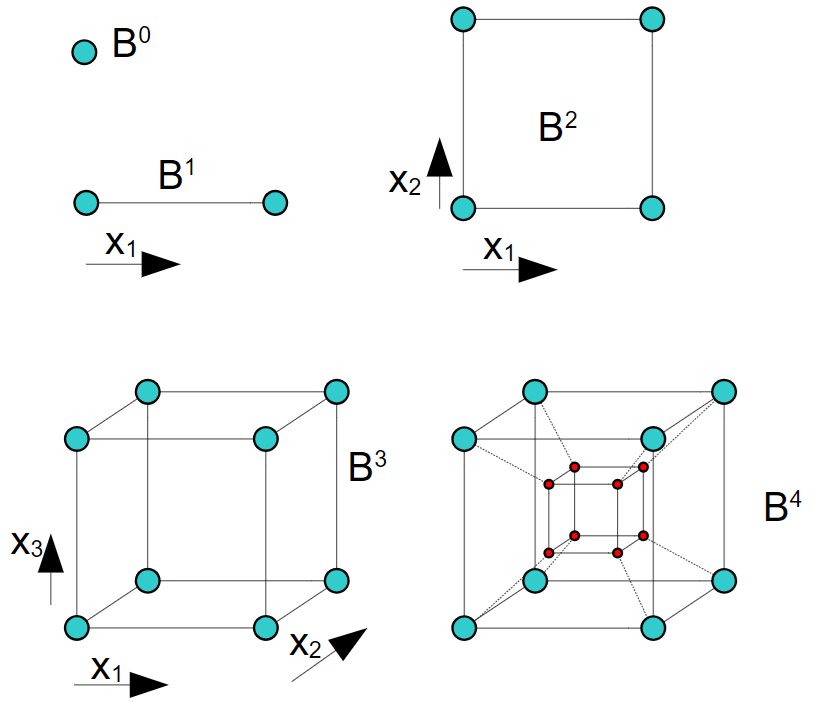
\includegraphics[width=\textwidth]{fig/krychle.png}
				\end{center}		
      
		\end{minipage}
		\begin{minipage}[t][\textheight][t]{0.45\textwidth}

			\begin{itemize}
				\item Kombinace odpovídají vrcholům krychle,
				\item šipky ukazují přechod z 0 do 1,
				\item sousední vrcholy se liší jen v hodnotě jedné proměnné, můžeme ji tedy použít pro minimalizaci,
				\item krychle není vhodným popisem pro více jak 3 proměnné - vícerozměrná krychle.
			\end{itemize}

		\end{minipage}

	\end{frame}

% =====================================================================================================================
	\begin{frame}
    \frametitle{Minimalizace pomocí krychle (\textbf{TEST!!!})}
		\boldmath
		
		\begin{minipage}[t][\textheight][t]{0.45\textwidth}
		
		\textbf{Viz pravdivostní tabulka výše:}
		\begin{center}
			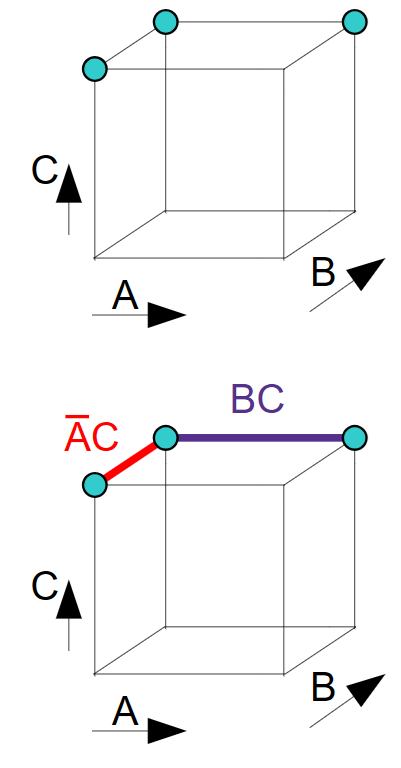
\includegraphics[width=0.6\textwidth]{fig/krychle_minimalizace.png}
		\end{center}
      
		\end{minipage}
		\begin{minipage}[t][\textheight][t]{0.45\textwidth}
    \vspace{10mm}
		
			\begin{itemize}
				\item Tvorba sousedních skupin jedničkových vrcholů,
				\item velikost skupiny musí být mocninou dvou: 1, 2, 4, 8
				\item do součinu se zapisuje proměnná, která v rámci prvků skupiny nemění hodnotu.
			\end{itemize}
    
		\vspace{5mm}
		$Y= \bar{A}C + BC$
		\end{minipage}
		
	\end{frame}
	
% =====================================================================================================================
	\begin{frame}
    \frametitle{Spínačová logika, liniové schéma}
		\boldmath
		
		\begin{minipage}[t][\textheight][t]{0.45\textwidth}
		\textbf{Základní prvky:}
		\begin{center}
			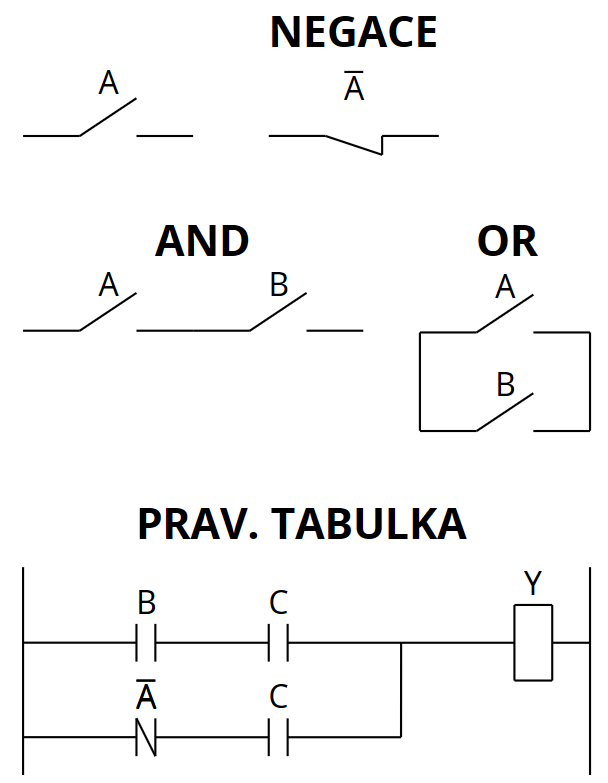
\includegraphics[width=0.9\textwidth]{fig/spinace.png}
		\end{center}
      
		\end{minipage}
		\begin{minipage}[t][\textheight][t]{0.45\textwidth}
    \vspace{10mm}
		
			\begin{itemize}
				\item Obsahuje všechny 3 operace Booleovské algebry,
				\item používá se pro návrh programu některých PLC,
			\end{itemize}
    
		\vspace{15mm}
		$Y= \bar{A}C + BC$
		\end{minipage}
		
	\end{frame}
	
% =====================================================================================================================
	\begin{frame}
    \frametitle{Karnaughova mapa}
		\boldmath
		
		\begin{minipage}[t][\textheight][t]{0.48\textwidth}
		\vspace{5mm}
		\textbf{Viz pravdivostní tabulka výše:}
		
		\begin{karnaugh-map}[4][2][1][$B$][$C$][$A$]
			\minterms{2,3,7}

			% ====== vlastní čáry ======

			% A = 1 (druhý řádek)
			\draw[very thick] (-0.15,1) -- (-0.15,0);

			% B = 1 (sloupce 3 a 4)
			\draw[very thick] (2,2.15) -- (4,2.15);

			% C = 1 (sloupce 2 a 3)
			\draw[very thick] (1,2.3) -- (3,2.3);

		\end{karnaugh-map}
      
		\end{minipage}
		\begin{minipage}[t][\textheight][t]{0.45\textwidth}
    \vspace{10mm}
		
			\begin{itemize}
				\item Obsahuje výčet všech kombinací,
				\item sousední vrcholy se liší jen v hodnotě jedné proměnné, můžeme ji tedy použít pro minimalizaci,
				\item snadná minimalizace až do 4 proměnných.
			\end{itemize}
    
		\end{minipage}
		
	\end{frame}
	
% =====================================================================================================================
	\begin{frame}
    \frametitle{Karnaughova mapa - minimalizace}
		\boldmath
		
		\begin{minipage}[t][\textheight][t]{0.48\textwidth}
		\vspace{5mm}
		\textbf{Viz pravdivostní tabulka výše:}
		
		\begin{karnaugh-map}[4][2][1][$B$][$C$][$A$]
			\minterms{2,3,7}
			\implicant{3}{2}
			\implicant{3}{7}

			% ====== vlastní čáry ======

			% A = 1 (druhý řádek)
			\draw[very thick] (-0.15,1) -- (-0.15,0);

			% B = 1 (sloupce 3 a 4)
			\draw[very thick] (2,2.15) -- (4,2.15);

			% C = 1 (sloupce 2 a 3)
			\draw[very thick] (1,2.3) -- (3,2.3);

		\end{karnaugh-map}
      
		\end{minipage}
		\begin{minipage}[t][\textheight][t]{0.45\textwidth}
    \vspace{10mm}
		
			\begin{itemize}
				\item Tvoříme sousední skupiny v mocninách 2,
				\item součástí součinu jsou jen proměnné, které v rámci skupiny nemění hodnotu,
				\item každá 1 musí být členem nejméně jedné skupiny.
			\end{itemize}
			
		\vspace{5mm}
		$Y=$ \textcolor{red}{$\bar{A}C$} $+$ \textcolor{green}{$BC$}
    
		\end{minipage}
		
	\end{frame}
